% !TeX spellcheck = en_GB
\documentclass[main.tex]{subfiles}

\begin{document}
\chapter{Methods}
\lhead{Methods}

\section{Pretrained LUKE model}
LUKE (Language Understanding with Knowledge-based Embeddings) is a language model introduced by Yamada et al. in November of 2020. \cite{yamada2020luke}.
As the model is tested and extended in this project, key properties of the architecture and pretraining methodology are presented in this section.

While architecturally similar to models such as BERT \cite{devlin2019bert} and RoBERTa \cite{liu2019roberta}, LUKE not only produces contextualized word representations (CWR), but also contextualized entity representations (CER), which, as Yamada et al. show, leads to state-of-the-art results on a number of entity-related tasks.

BERT \cite{devlin2019bert} and RoBERTa \cite{liu2019roberta} yield strong, general-purpose CWR's that are effective for many different NLP tasks but are often suboptimal for entity-related tasks.
Yamada et al. suggest three reasons for this being the case.
\begin{itemize}
    \item Existing CWR's include no span-level representation of entities, so these will have to be learned from a often small downstream dataset.
    \item While transformers are good at capturing relationships between single words, they have difficulty modelling such relationships between sequences of words, of which entities often consist.
    \item Finally, the word-based pretraining task is not suited for producing entity-level representations, as the masked language model (MLM) mostly learns to predict single words rather than entire entity spans.
    An example is predicting "Flies" in "Lord of the [MASK]", where predicting the single word is clearly easier than predicting the entire entity.
\end{itemize}
LUKE, in contrast to BERT and RoBERTa, also considers entities as tokens, and it takes and inputs both word and entity tokens and produces both CWR's and CER's, respectively.
This allows LUKE to deal with the listed problems of purely word-based language models.

\subsection{Architecture}
LUKE is a transformer that operates on input sequences using trainable word and entity embeddings which are encoded by 24 self-attention transformer layers.
After these, the model can be extended with a decoder consisting of bi-directional classifications heads for pretraining, or it can be extended with linear layers for downstream tasks.

\subsubsection{BERT Architecture}
The word/entity duality of LUKE means that a large part of the model performs the same task as the conventional word-based language models.
For this reason, the word embeddings in LUKE follow the BERT architecture and Yamada et al. initialize these embeddings to those found in RoBERTa.
In the pre-training of Yamada et al., the encoder of LUKE is also equivalent with that of BERT and is initialized the weights of RoBERTa.

\subsubsection{Entity Embeddings}
The only architectural difference between LUKE and BERT in the pretraining of Yamada et al. (apart from pretraining specific heads) is the addition of a map from entity id's and entity position id's to entity embeddings.
This part of the model consists of lookup tables that store values for each possible id.
For the entity token id embedding, the size of the lookup table corresponds to the size of the entity vocabulary.

The entity embeddings are concatenated to the word embeddings and are passed through the encoder such that the two token domains exist in the same latent space.
After the encoding, the output can be split into representations for the words and entities in the sequence.


\subsubsection{Entity-aware Self-attention}
\label{subsubsec:entityaware}
Yamada et al. present a entity-related change to the BERT encoder architecture in the query metchanism of the attention scorer \cite[Sec. 3.2]{yamada2020luke}.

For the attention between token $i$ and token $j$ with the hidden states $\mathbf x_i, \mathbf x_j$, a core part of the normal transformer attention mechanism is to compute the following scalar:
\begin{equation}
    q_{ij} = \mathbf x_j^\top \mathbf Q \mathbf x_i,
\end{equation}
where $\mathbf Q\in \RR^{H\low{in}\times H\low{out}}$ is called the query matrix for a layer with input hidden size $H\low{in}$ and output hidden size $H\low{out}$ \cite[Sec. 3.2.1]{vaswani2017att}.
% FIXME: H_in og H_out må da være det samme?

In LUKE, the tokens $\mathbf x_i$ might either be words or entities.
To handle this explicitly, entity-aware self-attention changes the computation of the scalar $q_{ij}$ to
\begin{equation}
    q_{ij} = 
    \begin{cases}
    \mathbf x_j^\top \mathbf Q_{w2w} \mathbf x_i  & \text{if both $\mathbf x_i$ and $\mathbf x_j$ are word tokens}\\
    \mathbf x_j^\top \mathbf Q_{w2e} \mathbf x_i & \text{if $\mathbf x_i$ is word and $\mathbf x_j$ is entity}\\
    \mathbf x_j^\top \mathbf Q_{e2w} \mathbf x_i & \text{if $\mathbf x_i$ is entity and $\mathbf x_j$ is word}\\
    \mathbf x_j^\top \mathbf Q_{e2e} \mathbf x_i & \text{if both $\mathbf x_i$ and $\mathbf x_j$ are entity tokens}
    \end{cases}
\end{equation}
LUKE, however, is not pretrained using this mechanism, but for the fine-tuning tasks, Yamada et al. show in ablation experiments that this addition consistently yields better performance \cite[Sec. 5.2]{yamada2020luke}.

\subsection{Pretraining}
Yamada et. al perform the pretraining of LUKE by extending the MLM task of BERT \cite{devlin2019bert}.
Where BERT is trained to predict randomly masked words, LUKE is trained to predict both randomly masked words and entities.

The pretraining task thus gives three sequences as input:
Word id's, entity id's, and positions of the entities.
15\pro\ of words and entities are randomly replaced by the [MASK] token, following RoBERTa \cite{liu2019roberta}.
From these, the model is to classify the tokens at the mask positions in both sequences.
The model parameters are then updated by the AdamW optimizer backpropagating through loss computed as the sum of the multi-class cross entropy losses of the two classification tasks.

\subsubsection{Entity Mask Prediction Head}
For the entity pretraining task, LUKE is equipped with another classifier structure in addition to the masked language model prediction head inherited from BERT.
This new prediction head follows the architecture of the masked word scorer just operating on the entity representations.
The masked entity tokens are thus scored as corresponding to one of the entities in the entity vocabulary by two linear layers between which an activation function and layer normalization are placed.


\section{Benchmarking Existing Named Entity Recognition}
\subsection{Fine-tuning English LUKE}
Yamada et al. benchmark \emph{LUKE}, their new transformer-based model for contextualized entity representations on a number of Natural Language Processing tasks, including Named Entity Recognition on the CoNLL-2003 dataset \cite{yamada2020luke}.

Reproduction of these results were performed by obtaining the pretrained LUKE models from Yamada et al.'s software repository.

The model was then fine-tuned for NER by training a linear classifier over all $n$-grams in each sentence with the named entities as targets for cross-entropy loss, as described in \cite[Sec. 4.3]{yamada2020luke}.
The same hyper-parameters as Yamada et al. were used and are shown along with and technical details in Table~\ref{tab:params}.

This procedure was repeated five times for each of the two released LUKE models, called \emph{large} and \emph{base}, to examine variability in the downstream training.

%%% Horrible footnote manipulation - it works, dont touch it! %%%
\addtocounter{footnote}{1}
\footnotetext{\label{foot:fnt}
    The pre-trained models were downloaded on 17/02-2021 from the LUKE software repository:
    \url{https://github.com/studio-ousia/luke/tree/6feefe657d97d2f847ace87f61f23b705f75d2aa\#released-models} 
} 
\begin{table}[H]
    \begin{tabular}{l|cc}
                                    & LUKE large & LUKE base\\\hline
        Pre-trained model
                                    & LUKE RoBERTa large \textsuperscript{\ref{foot:fnt}}\
                                                & LUKE RoBERTa base\textsuperscript{\ref{foot:fnt}}\\
        Pre-trained model parameters & $253\ctp 6$ & $483\ctp 6$\\
        Pre-trained model entity vocabulary & \multicolumn{2}{c}{$500\ctp3$}\\
        Learning rate               & $10^{-5}$ & $5\ctp{-5}$\\
        Batch size (effective)      & \multicolumn{2}{c}{8 (16)}\\
        Gradient accumulation steps & \multicolumn{2}{c}{2}\\
        Numeric precision           & \multicolumn{2}{c}{Mixed FP16/FP32 (Nvidia APEX)}\\
        Training code               & \multicolumn{2}{c}{PyTorch-based \code{luke}-repository \protect\footnotemark}\\
        Software version            & \multicolumn{2}{c}{Python 3.6, PyTorch 1.2}
    \end{tabular}
    \label{tab:params}
\end{table}

\footnotetext{
    The repository \url{github.com/studio-ousia/luke} was cloned at commit-SHA \code{6feefe6}, installed and used for the fine-tuning.
}
\subsection{Off-the-shelf, Danish models}
\label{sec:exidan}
A number of Danish NER models that are publily available and usable by NLP practitioners are collected and evaluated on the testing datasets of three Danish NER annotations considered in \ref{subsec:daNERdata}: DaNE, Plank and Wiki-ANN.

Most of the models are found through DaNLP\footnotemark, an open-source collection of Danish NLP software and references released by the Alexandra Institute which also released the DaNE dataset.
\footnotetext{
    The repository is at \url{https://github.com/alexandrainst/danlp} from which a collection of NER models can be found under \code{docs/docs/tasks/ner.md}.
}\\
\\
\textbf{DaNLP da-BERT}
is an NER model produced by DaNLP by using the pretrained Danish BERT released by the company BotXO \cite{botxo2019dabert} under the Creative Commons 4.0 open source license.
The model is fine-tuned for NER on the DaNE test set \cite{hvingelby2020dane}.\\
\\
\textbf{NERDA m-BERT}
is a NER model fine-tuned by Ekstra Bladet Analyse in their repository NERDA\footnotemark, \emph{NER for Danish} using the pre-trained Multilingual BERT released by the original Google Research BERT team \cite{devlin2019bert}.
The training data was also DaNE.
\footnotetext{
    The repository is at \url{https://github.com/ebanalyse/NERDA}.
}\\
\\
\textbf{NERDA Ælæctra}
is also released in the NERDA repository and uses the Danish Transformer Ælæctra which has been pre-trained on the Danish Gigaword Corpus by Malte Højmark-Bertelsen at KMD \cite{bertelsen2020lctra}.
The model is an adaption of the efficient BERT alternative Electra \cite{clark2020electra} and has been fine-tuned by NERDA on DaNE.\\
\\
\textbf{DaNLP Flair}
is a NER model based on the open-source contextual word embedding framework Flair \cite{akbik2019flair}, fine-tuned on DaNE by DaNLP.\\
\\
\textbf{DaNLP spaCy}
is a model released in DaNLP which is obtained by training the general, open-source NLP framework spaCy \cite{honnibal2020spacy} on the Universal Dependencies Danish Dependency Treebank (UD-DDT) Corpus\cite{johann2015udddt}.
This Danish spaCy model was then fine-tuned for NER on DaNE.\\
\\
\textbf{Polyglot}
is a NLP framework supporting a wide range of tasks in many languages including NER in 40 different languages.
The NER model is produced using automatic, language-agnostic annotations generated from Wikipedia and Freebase link structures \cite{rfou2015polyglot}.\\
\\
\textbf{DKIE Stanford CRF (daner)}
is an application of the Stanford CoreNLP Conditional Random Field (CRF) NER classifier \cite{manning2014corenlp} released by IT University of Copenhagen (ITU).
The model was trained on NER annotations produced at ITU on the Danish Dependency Treebank (DDT) corpus \cite{kromann2003ddt} as a part of the DKIE project \cite{derc2014dkie}.
The released Java-based NER tool is called \code{daner}\footnotemark.
\footnotetext{
    The repository is at \url{https://github.com/ITUnlp/daner}
}
%TODO Tilføj dacy

\section{DaLUKE}

% Vi bruger enitetsopmærksom
% Andre ting, vi lige kommer på
\subsection{Pretraining Methodology and Hyperparameters}%
\label{sub:dalpre}
DaLUKE's pretraining largely follows LUKE's with some differences:
\begin{itemize}
    \item The entity-augmented Danish Wikipedia described in section \ref{subsec:entaug} is used.
    \item Entity-aware self-attention is used for the pretraining.
    \item Weights are initialized from da-BERT.
    All four attention matrices described in section \ref{subsubsec:entityaware} are initialized to the same attention matrix in da-BERT.
    \item The full entity vocabulary is used.
\end{itemize}
Due to the memory intensive nature of the transformer architecture, we follow Yamada et al. and use gradient accumulation over multiple subbatches within each batch.

The learning rate, which uses a linear warmup followed by a linear decay, is updated after each batch.
This prevents the model from overfitting on early examples and allows better optimization later on, while still retaining a relatively high learning rate throughout of most the training, without the training dragging on, as it would with a constant, low learning rate.

%TODO Overvej: Skal dette ned i implementeringsdetaljer?
The model is trained using Pytorch Automatic Mixed Precision (AMP) \cite{pytorchamp}, which -- ideally, at least, as will be discussed in section \ref{sub:oss} -- should decrease training time with little to no penalty to accuracy. \cite{huang2020amp}
This is partially due to half-precision calculations being simpler, and partially due to the lower memory requirements, allowing larger subbatches and thus better GPU utilization.
However, as figure \ref{fig:runtime} shows, AMP works as intended when training on NVIDIA V100's, but has the opposite effect when training on NVIDIA A100's.

\noindent
The hyperparameters used for pretraining are shown in table \ref{tab:pretrain-hyper}.
\begin{table}[H]
    \centering
    \begin{tabular}{l|r}
        Parameter  &    Value\\\hline
        Epochs     & 150\\
        Batch size &    4080\\
        Peak learning rate & $5\ctp{-4}$\\
        LR warmup steps prop. & $ 6\pro $\\
        Mask prob. for words & $ 15\pro $\\
        Mask prob. for entities & $ 15\pro $\\
        Dropout & $ 0.1 $\\
        Weight decay & $ 0.01 $\\
        AdamW $ \beta_1 $ & $ 0.9 $\\
        AdamW $ \beta_2 $ & $ 0.999 $\\
        AdamW $ \epsilon $ & $ 10^{-6} $
    \end{tabular}
    \caption{Hyperparameters for DaLUKE pretraining.}\label{tab:pretrain-hyper}
\end{table}\noindent

\subsection{Fine-tuning daLUKE for Named Entity Recognition}%
\label{sub:finetune-ner}


\subsection{Implementation Details and Open Source Software}%
\label{sub:oss}

\subsubsection*{Training Time and GPU details}
As transformer training requires significant compute, distributing the training over multiple GPU's can yield significant speedups.
Especially given the parallelizable nature of the transformer compared to recurrent neural network variations \cite{vaswani2017att}, training should scale fairly well on multiple GPU's.

The pretraining took roughly a week.
Due to varying GPU availability, both A100's and V100's were used at different parts of the pretraining with $ 2\times $A100 being the most common configuration.
For comparison, Yamada et al. train LUKE using 16 V100's over a period of 30 days. \cite{yamada2020luke}

We measure the time needed to train for one epoch on different cluster configurations.
The results are shown on figure \ref{fig:runtime}.
\begin{figure}[H]
    \centering
    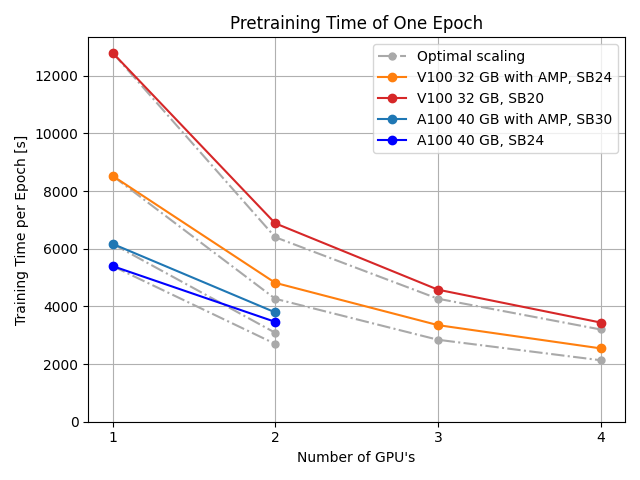
\includegraphics[width=.7\textwidth]{runtime}
    \caption{
        How GPU models, number of GPU's, and AMP influences pretraining runtime.
        Sub-batch size (SB) is included, as it is important for GPU utilization.
        The measurements were taken with da-BERT weights locked.
        The V100's act mostly as expected with close to optimal scaling and AMP decreasing runtime.
        Surprisingly, however, the A100's, while faster, scale poorly and are slower when using AMP.
        While we cannot offer an explanation for this behaviour, we suspect it may be due to different hardware other than the GPU's, driver versions, or CUDA versions.
        PyTorch 1.8.1 compiled with CUDA 11.1 was used.
    }
    \label{fig:runtime}
\end{figure}\noindent

\subsubsection{Distributed Training}



\end{document}
